\documentclass[a4paper]{article}
\usepackage{amsmath,amssymb,caption,float,graphicx,indentfirst,parskip,pdfpages,tabularx,xcolor}
\usepackage{hyperref}
% \usepackage{minted}
% \usepackage[utf8]{inputenc}
% \usepackage[english]{babel}
% \usepackage[backend=bibtex]{biblatex}
% \addbibresource{Lab3.bib}
\captionsetup[figure]{labelsep=period}
\captionsetup[listing]{labelsep=period}
% \definecolor{bg}{rgb}{0.95,0.95,0.95}
\hypersetup{
    colorlinks=true,
    linkcolor=blue,
    filecolor=blue,      
    urlcolor=blue,
    citecolor=cyan,
}
\setlength{\parindent}{2em}
% \usemintedstyle{emacs}
\begin{document}
\begin{titlepage}
    \vspace*{0.25cm}
    \noindent\rule[0.25\baselineskip]{\textwidth}{1pt}
    \begin{center}
        \huge{\textsc{UM--SJTU Joint Institute}}\vspace{0.3em}\\
        \huge{\textbf{System-on-Chip Design (ECE4810J)}}\vspace{0.3em}\\
        \noindent\rule[0.25\baselineskip]{\textwidth}{1pt}
    \end{center}
    \begin{center}
        \vspace{5cm}
        \Large{\textsc{Laboratory Report}}\vspace{0.5em}\\
        \Large{\textbf{Lab 4. Optimizing Performance through Pipelining}}\vspace{1em}\\
        \Large{\textbf{Group 2}}\\
    \end{center}
    \vfill
    \large
    \begin{tabular}{ll}
        Name: Haochen Wu \hspace*{2em}&ID: 518021910558\hspace*{2em}\\
        Name: Siyuan Zhang \hspace*{2em}&ID: 518370910180 \hspace*{2em}\\
        Name: Yihua Liu \hspace*{2em}&ID: 518021910998\hspace*{2em}\\
        \\
        Date: \today
    \end{tabular}
\end{titlepage}
\tableofcontents
\newpage
\section{Overview}
This is a lab for exercising the HLS flow on Zynq using Vivado. The goals of this lab are:
\begin{itemize}
    \item Understand the effect of INLINE directive
    \item Improve performance using PIPELINE directive
    \item Distinguish between DATAFLOW directive and Configuration Command functionality
\end{itemize}
\section{Optimizing Performance through Pipelining}
The PDF pages are the results given by Vitis HLS 2021.1 and the figures are the results given by Vivado HLS 2019.2. The PDF pages are converted from HTML files of Export Wizard by open-source tool \href{https://wkhtmltopdf.org/}{wkhtmltopdf}.
\subsection{Create a Vivado HLS Project from Command Line}
\subsection{Analyze the Created Project and Results}
\subsection{Apply TRIPCOUNT Pragma}
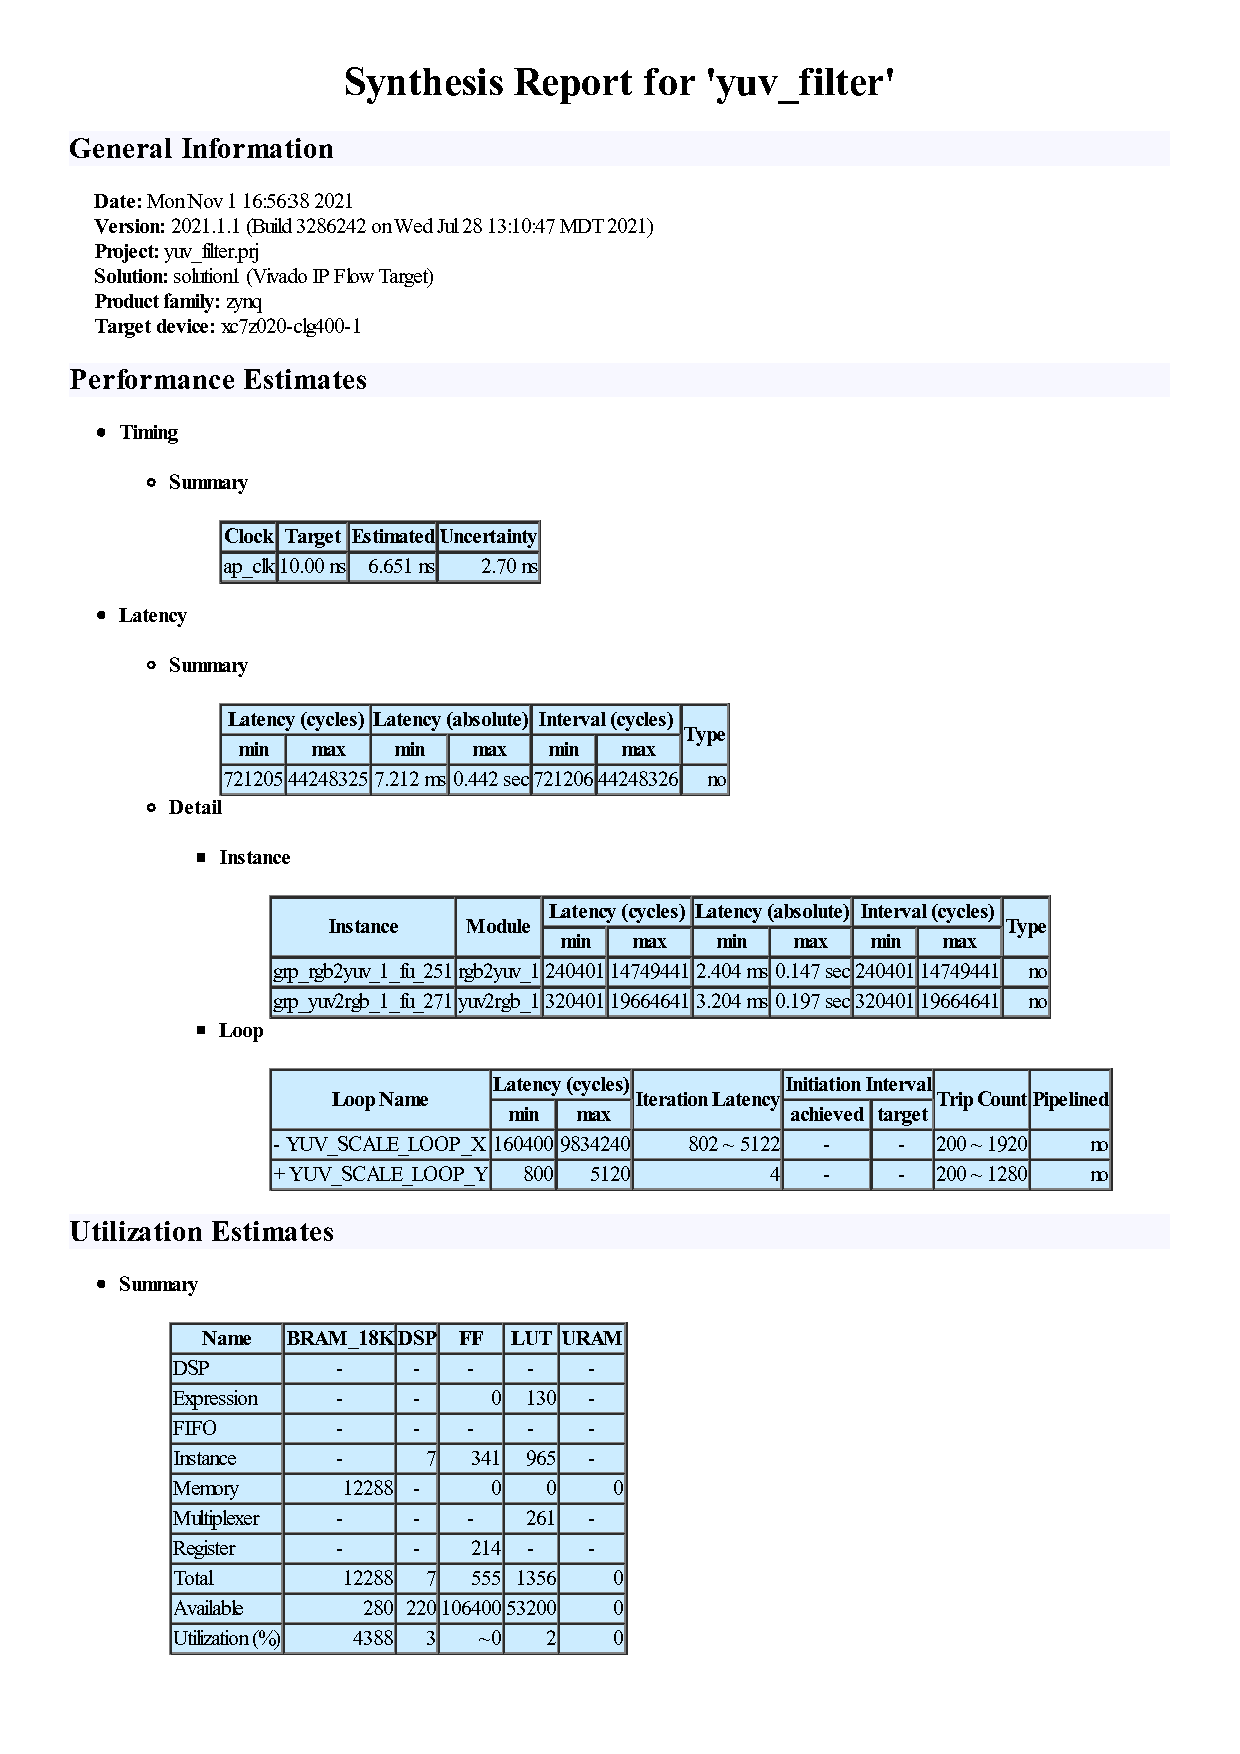
\includepdf[pages=1-4]{solution1_yuv_filter_csynth.pdf}

\begin{figure}[H]
    \centering
    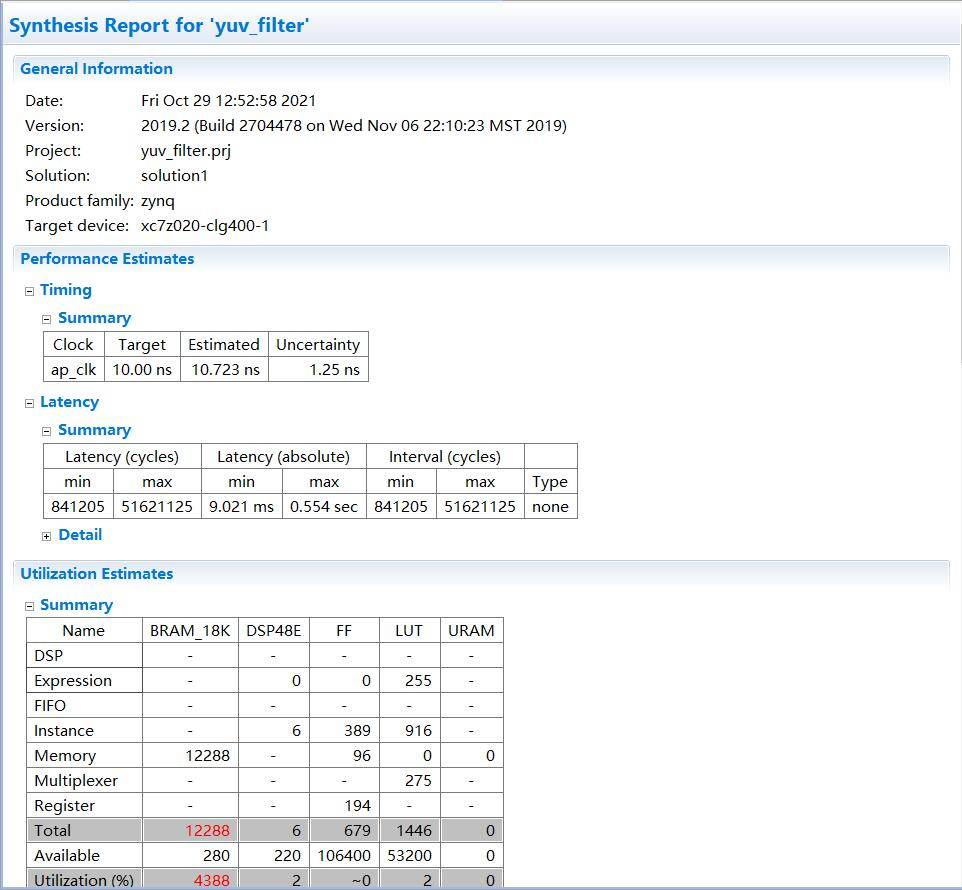
\includegraphics[width=1\textwidth]{1.jpg}
    \caption{In 2.3, Step 3.}
\end{figure}

\begin{table}[H]
    \centering
    \begin{tabular}{|c|c|c|}
        \hline
        Parameter&Vivado HLS 2019.2&Vitis HLS 2021.1\\
        \hline
        Estimated clock period&10.723\,ns&6.651\,ns\\
        \hline
        Worst case latency&0.554\,sec (51621125 cycles)&0.442\,sec (44248325 cycles)\\
        \hline
        Number of DSP48E used&6&7\\
        \hline
        Number of BRAMs used&12288&12288\\
        \hline
        Number of FFs used&679&555\\
        \hline
        Number of LUTs used&1446&1356\\
        \hline
    \end{tabular}
    \caption{Parameters of yuv\_filter function.}
\end{table}
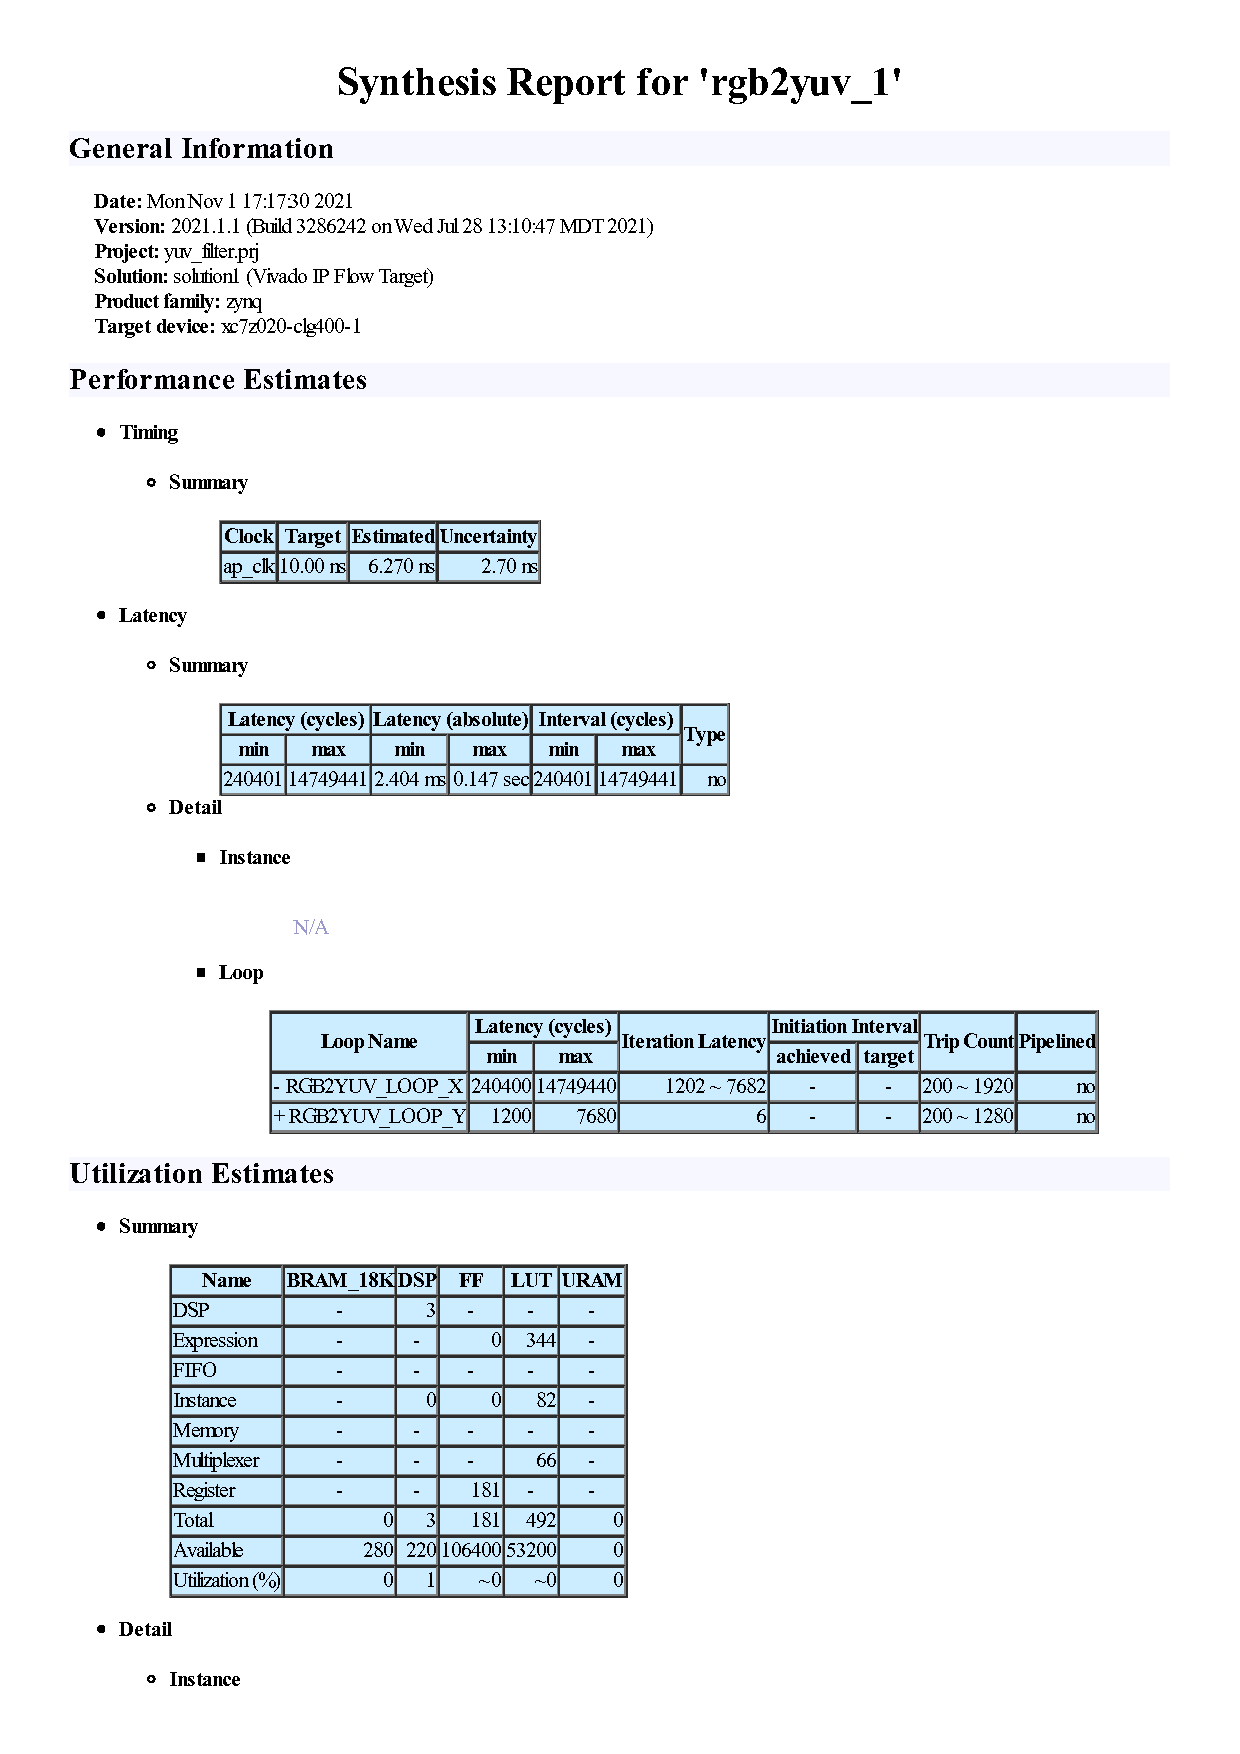
\includepdf[pages=1-3]{solution1_rgb2yuv_csynth.pdf}
\begin{figure}[H]
    \centering
    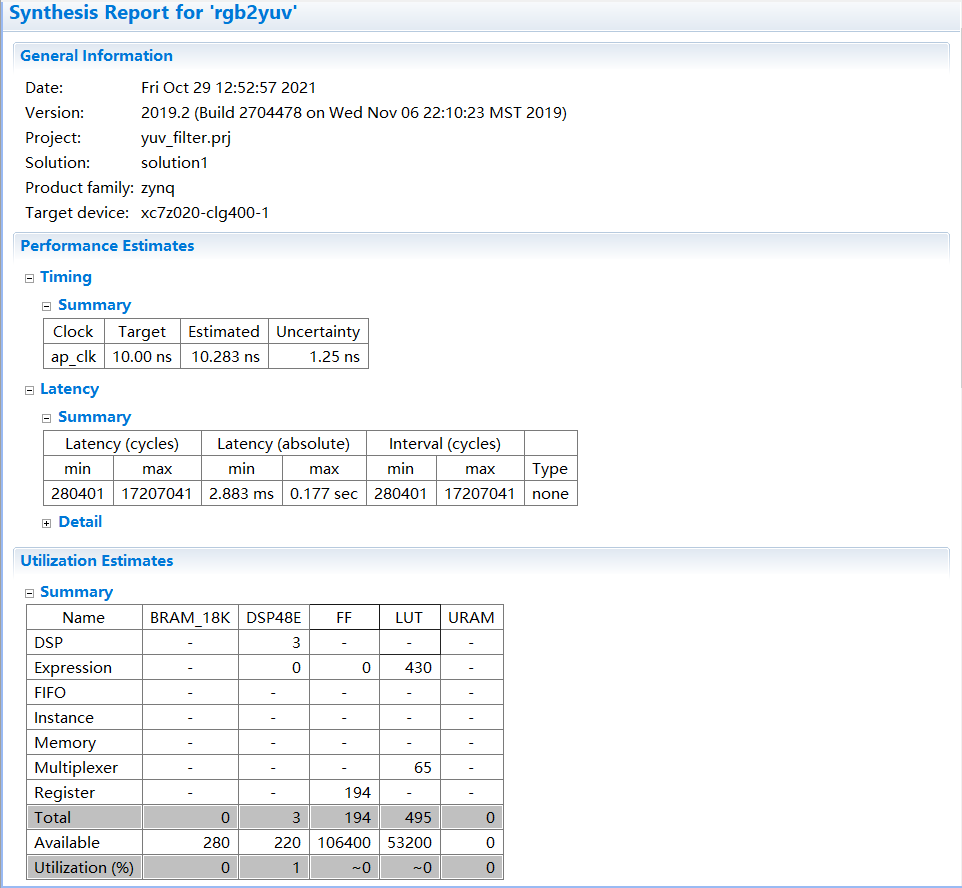
\includegraphics[width=1\textwidth]{2.png}
    \caption{In 2.3, Step 8.}
\end{figure}

\begin{table}[H]
    \centering
    \begin{tabular}{|c|c|c|}
        \hline
        Parameter&Vivado HLS 2019.2&Vitis HLS 2021.1\\
        \hline
        Estimated clock period&10.283\,ns&6.270\,ns\\
        \hline
        Worst case latency&0.177\,sec (17207041 cycles)&0.147\,sec (14749441 cycles)\\
        \hline
        Number of DSP48E used&3&3\\
        \hline
        Number of BRAMs used&0&0\\
        \hline
        Number of FFs used&194&181\\
        \hline
        Number of LUTs used&495&492\\
        \hline
    \end{tabular}
    \caption{Parameters of rgb2yuv function.}
\end{table}

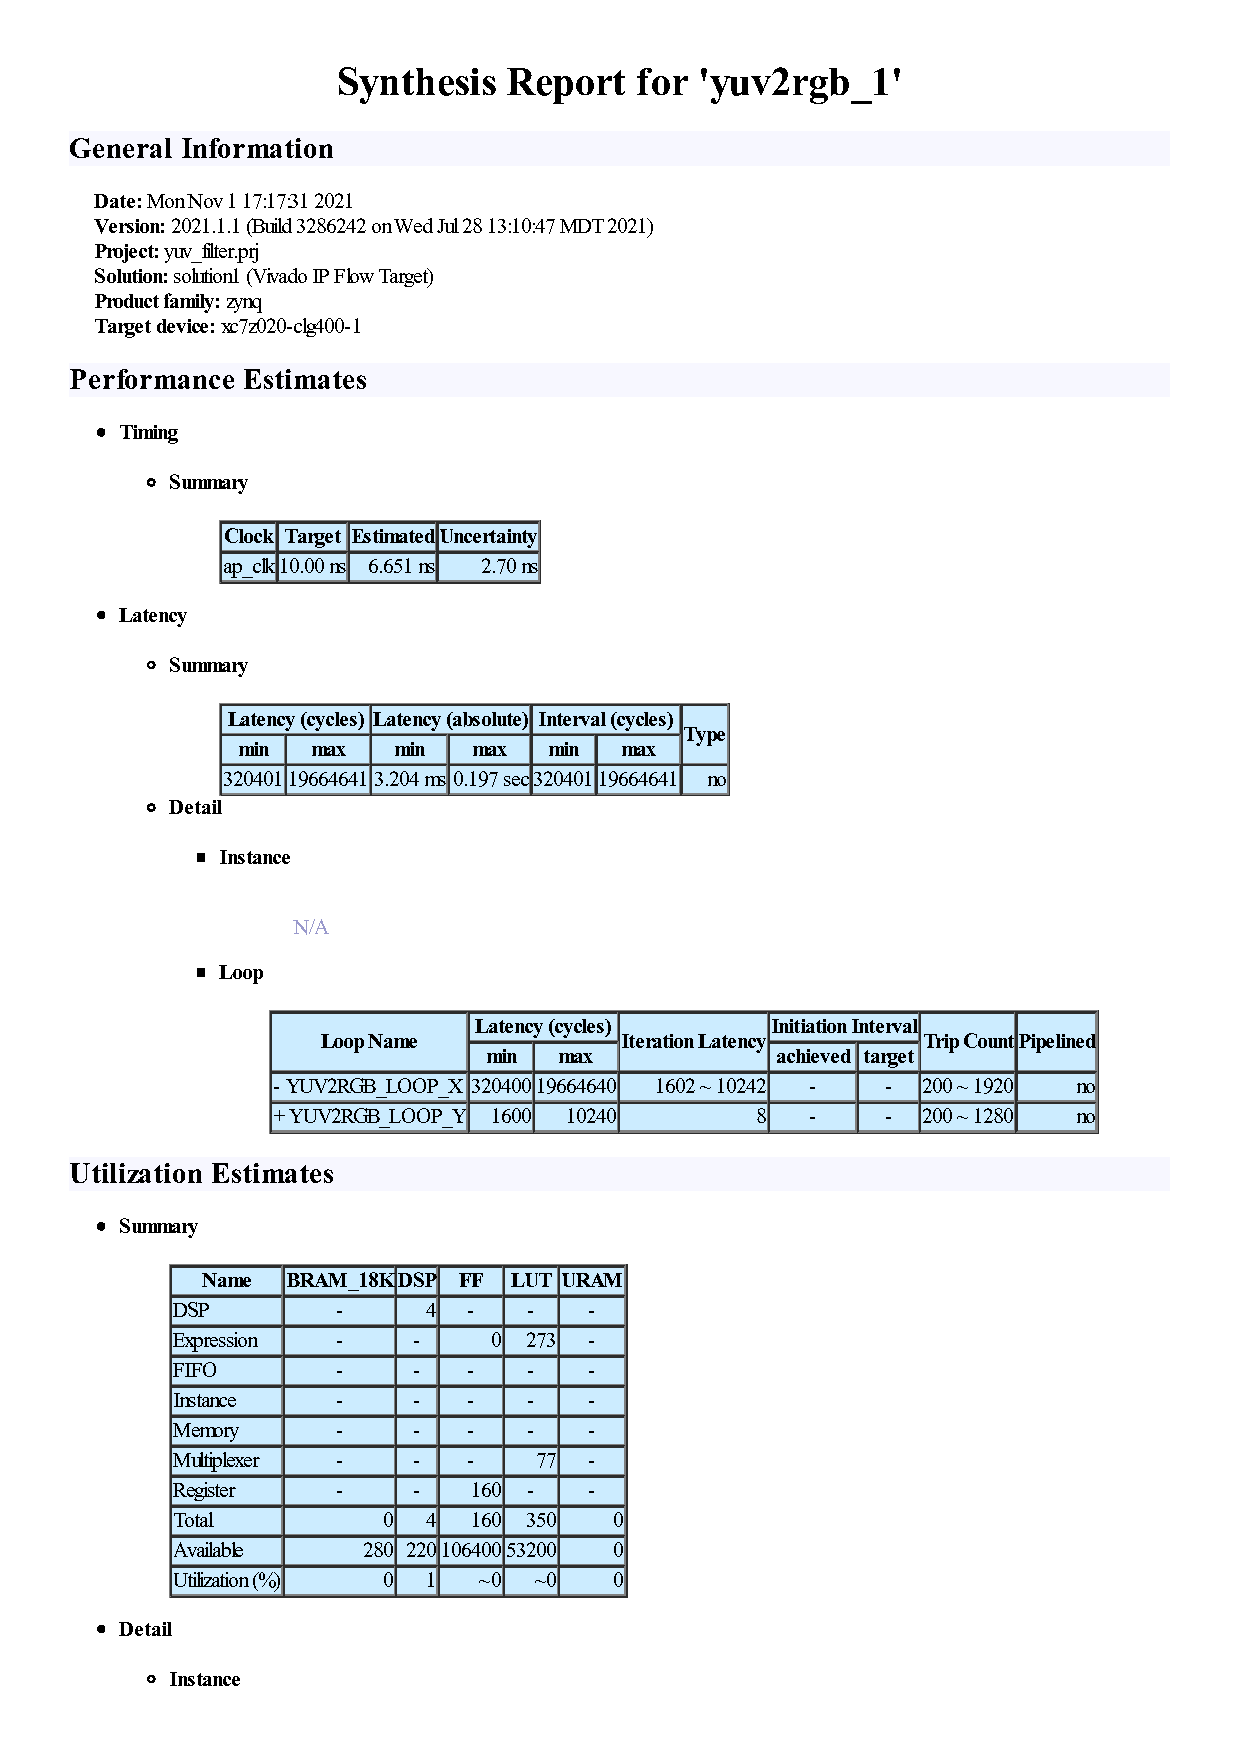
\includepdf[pages=1-3]{solution1_yuv2rgb_csynth.pdf}
\begin{figure}[H]
    \centering
    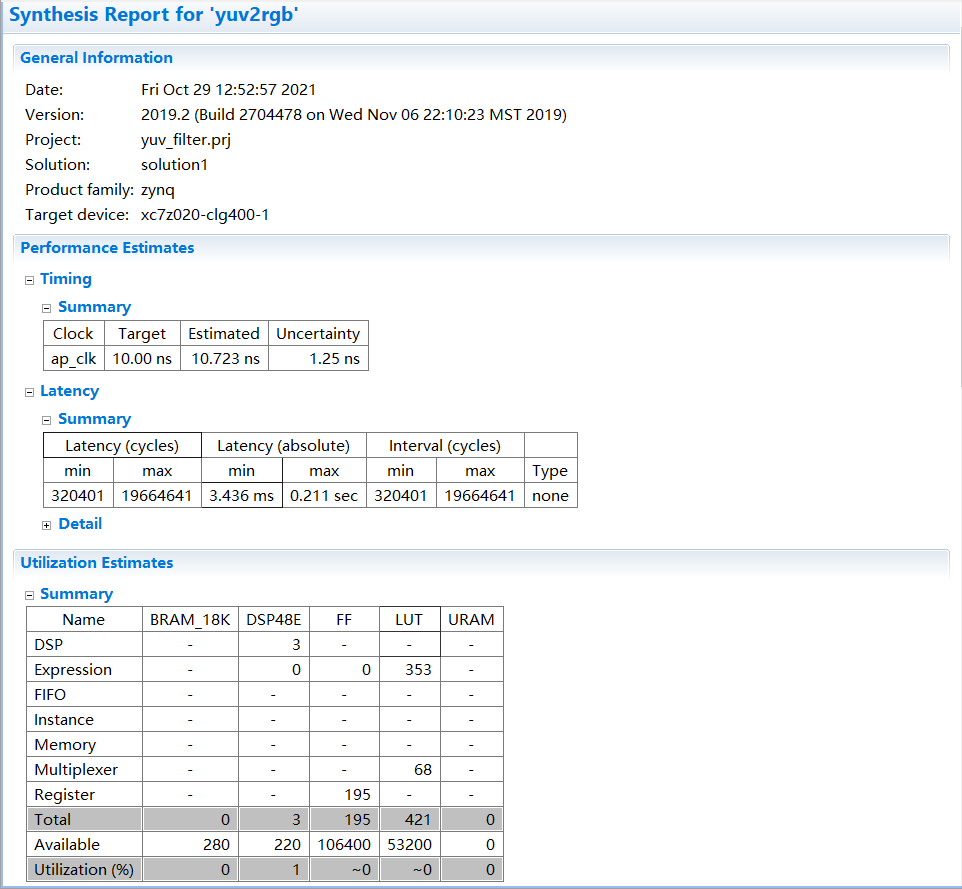
\includegraphics[width=1\textwidth]{3.png}
    \caption{In 2.3, Step 9.}
\end{figure}

\begin{table}[H]
    \centering
    \begin{tabular}{|c|c|c|}
        \hline
        Parameter&Vivado HLS 2019.2&Vitis HLS 2021.1\\
        \hline
        Estimated clock period&10.723\,ns&6.651\,ns\\
        \hline
        Worst case latency&0.211\,sec (19664641 cycles)&0.197\,sec (19664641 cycles)\\
        \hline
        Number of DSP48E used&3&4\\
        \hline
        Number of BRAMs used&0&0\\
        \hline
        Number of FFs used&195&160\\
        \hline
        Number of LUTs used&421&350\\
        \hline
    \end{tabular}
    \caption{Parameters of yuv2rgb function.}
\end{table}
\subsection{Turn OFF INLINE and Apply PIPELINE Directive}
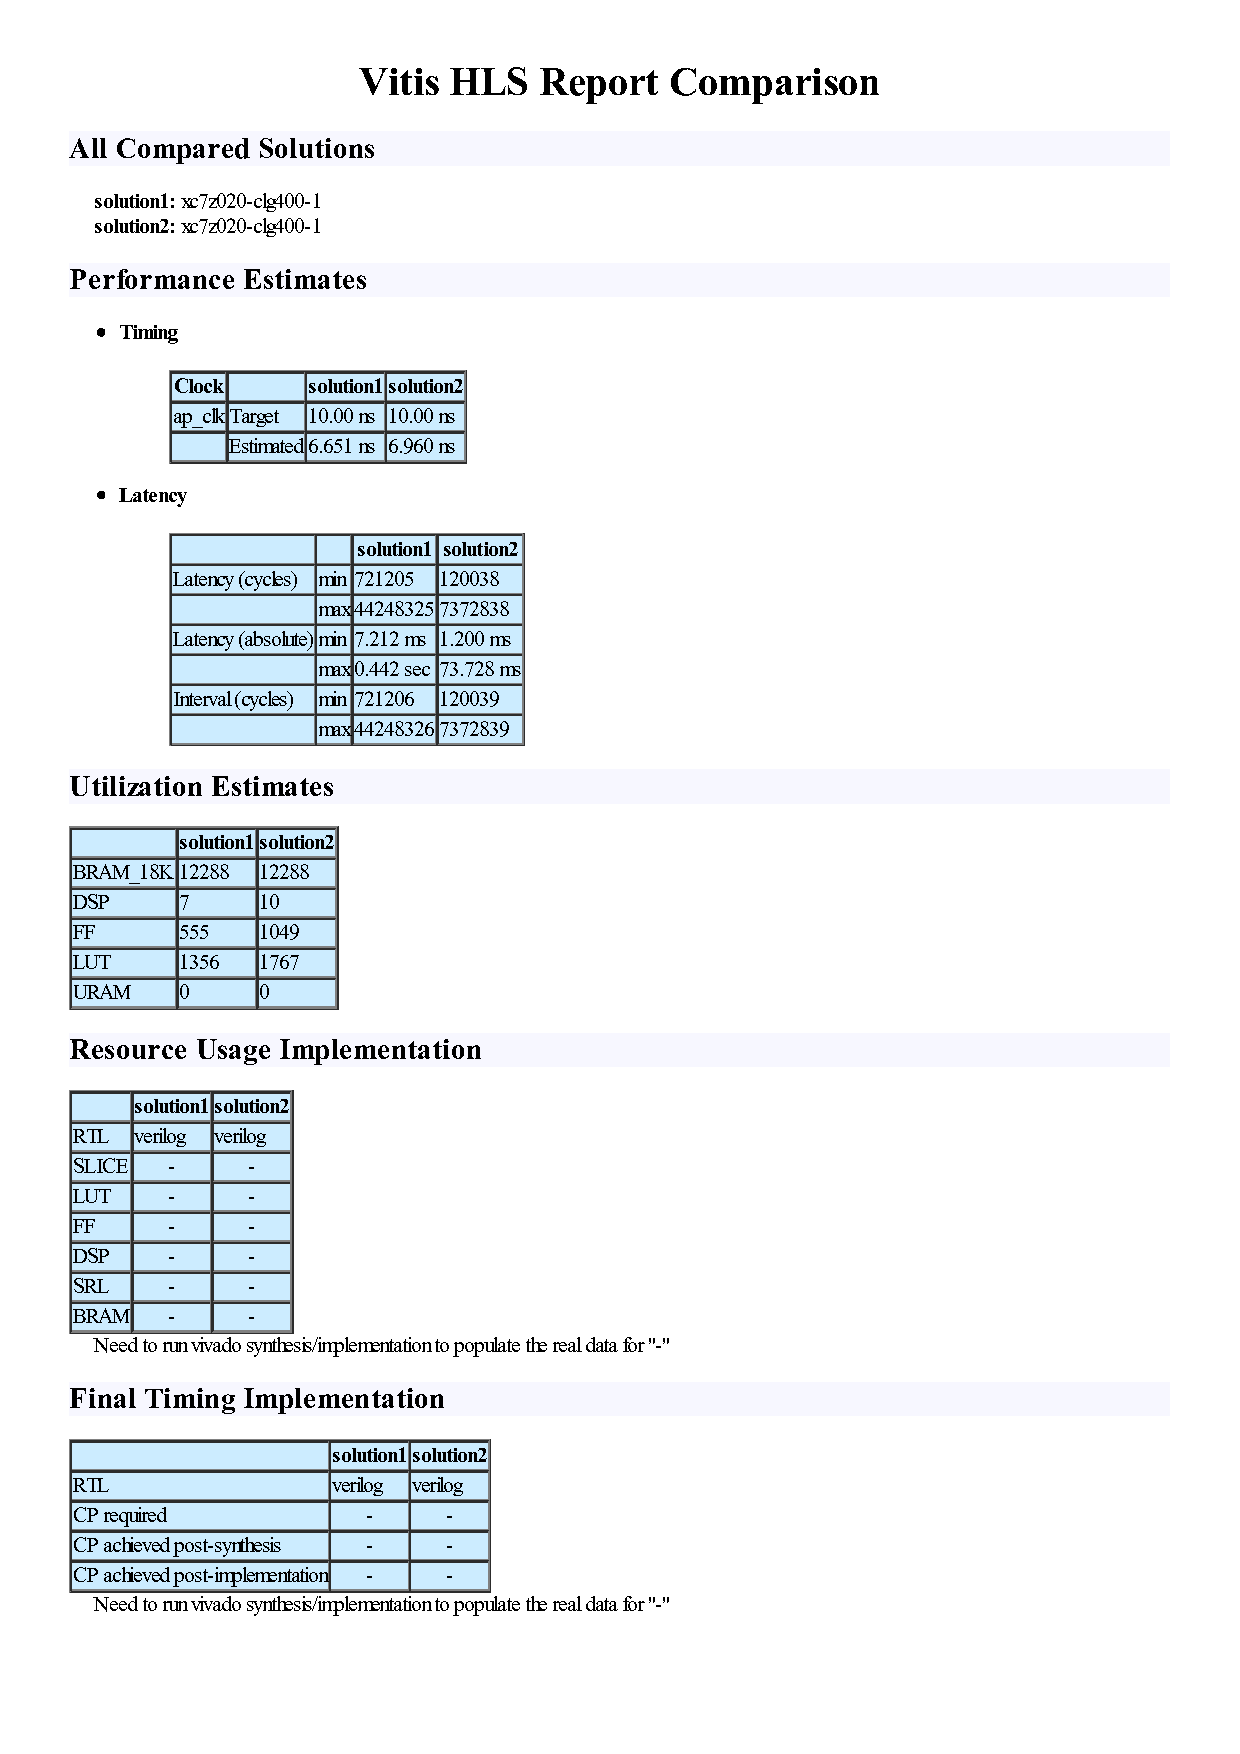
\includepdf{vitis_hls_compare_report.pdf}

\begin{figure}[H]
    \centering
    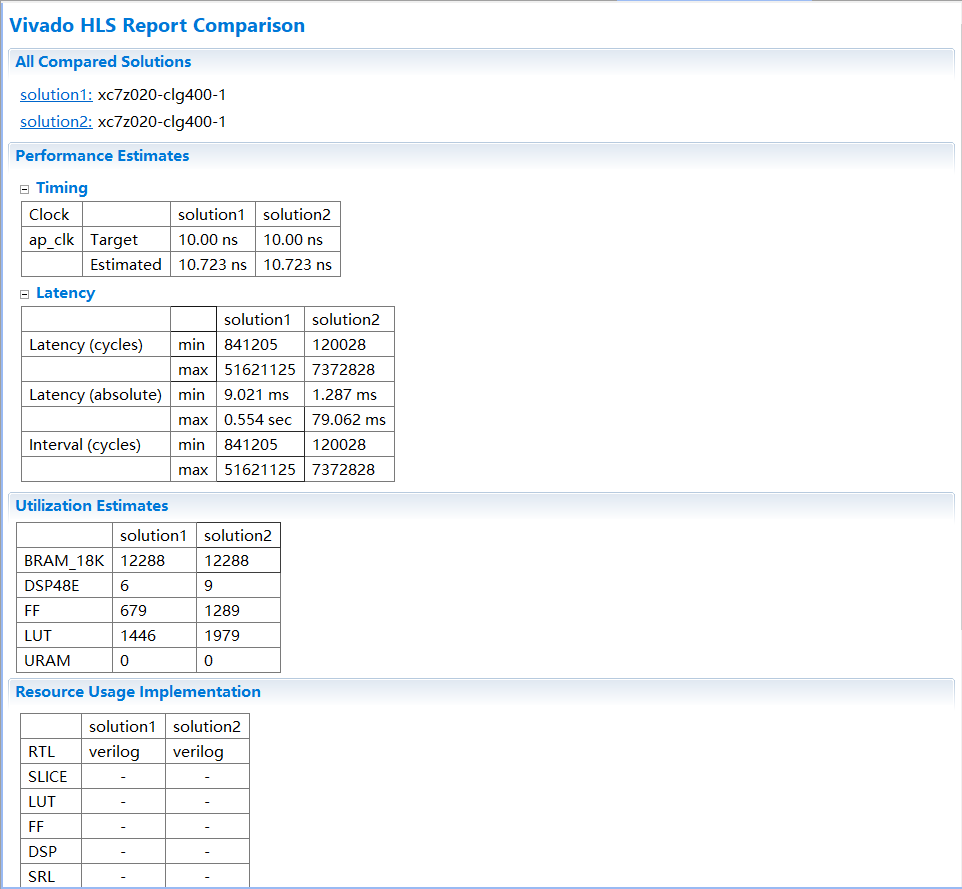
\includegraphics[width=1\textwidth]{4.png}
    \caption{In 2.4, Step 15, a screenshot of the resources utilization.}
\end{figure}
The FFs, LUTs, and DSP48E utilization increased whereas BRAM remained same.
\subsection{Apply DATAFLOW Directive and Configuration Command}
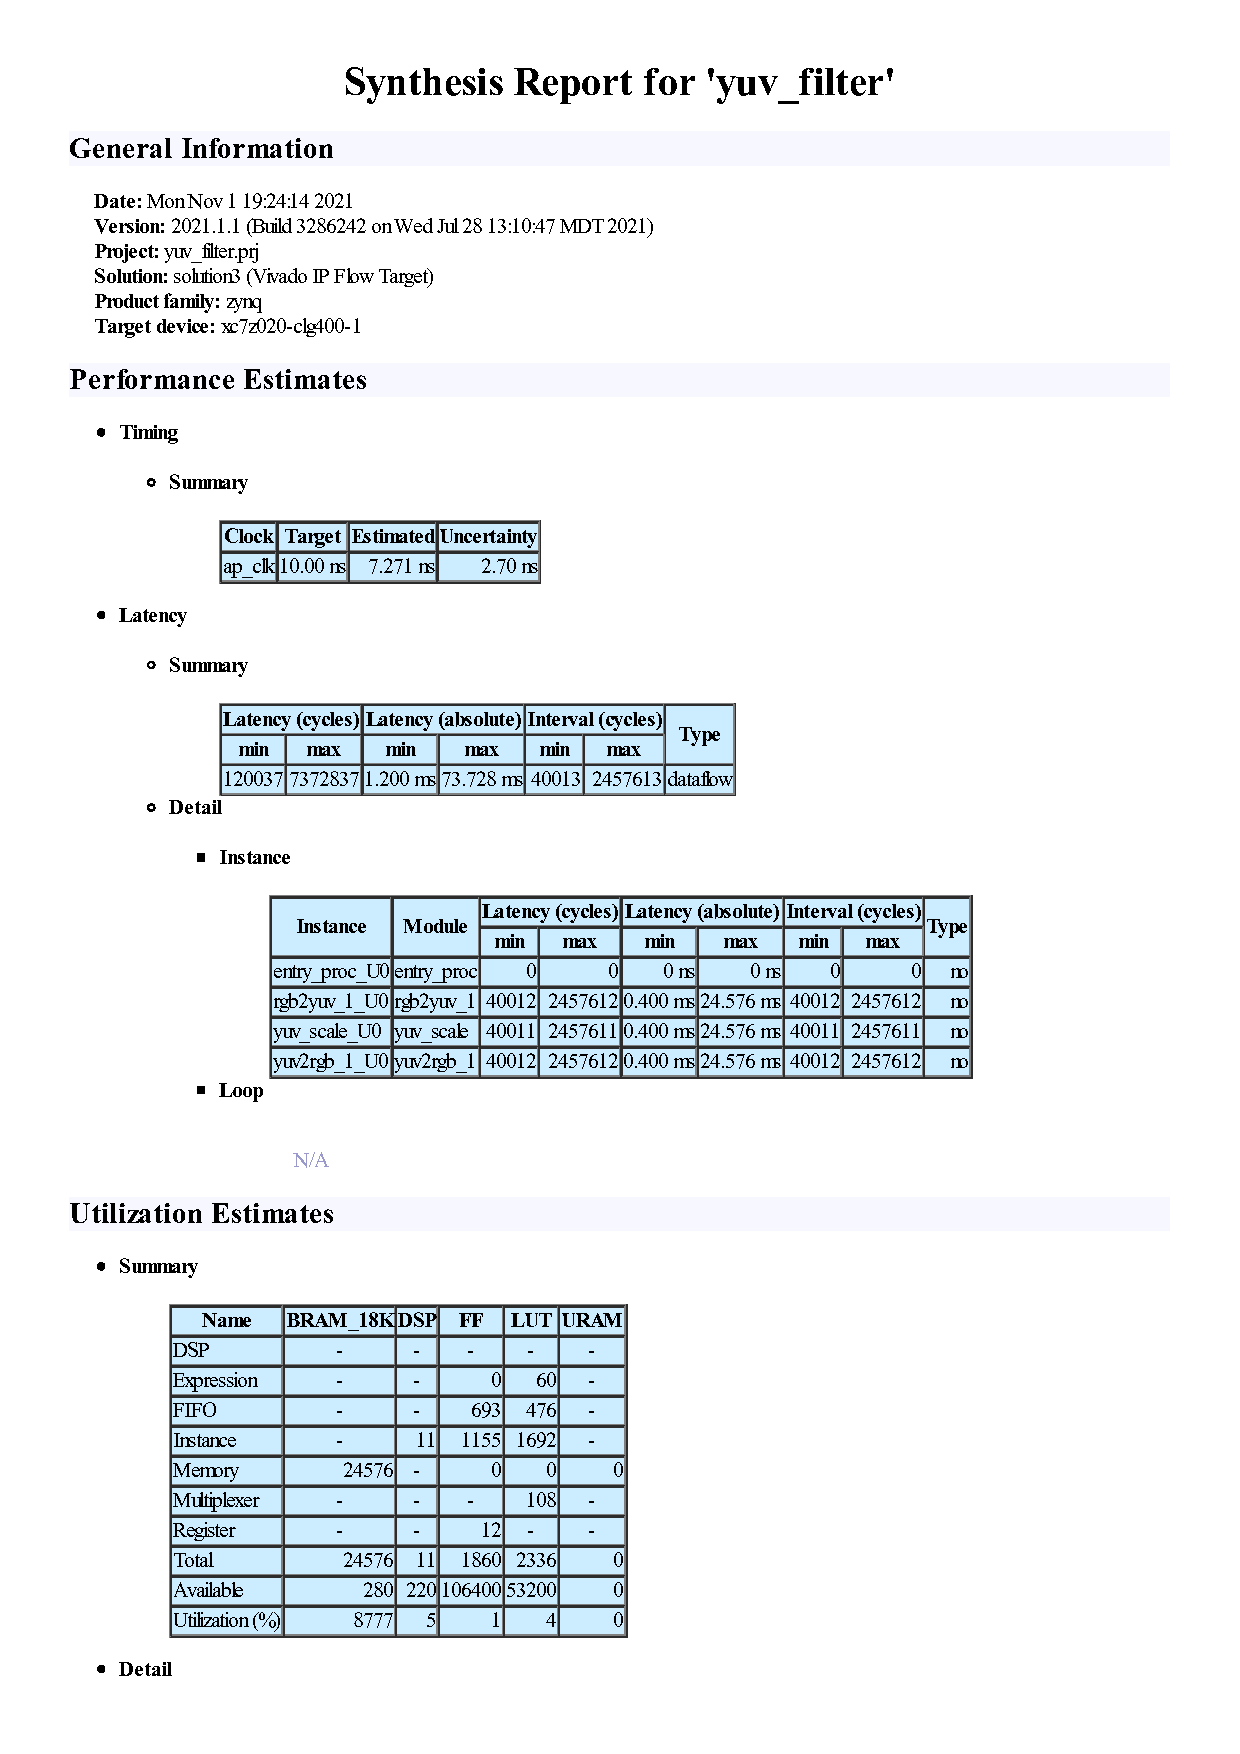
\includepdf[pages=1-5]{solution3_yuv_filter_csynth.pdf}
\begin{figure}[H]
    \centering
    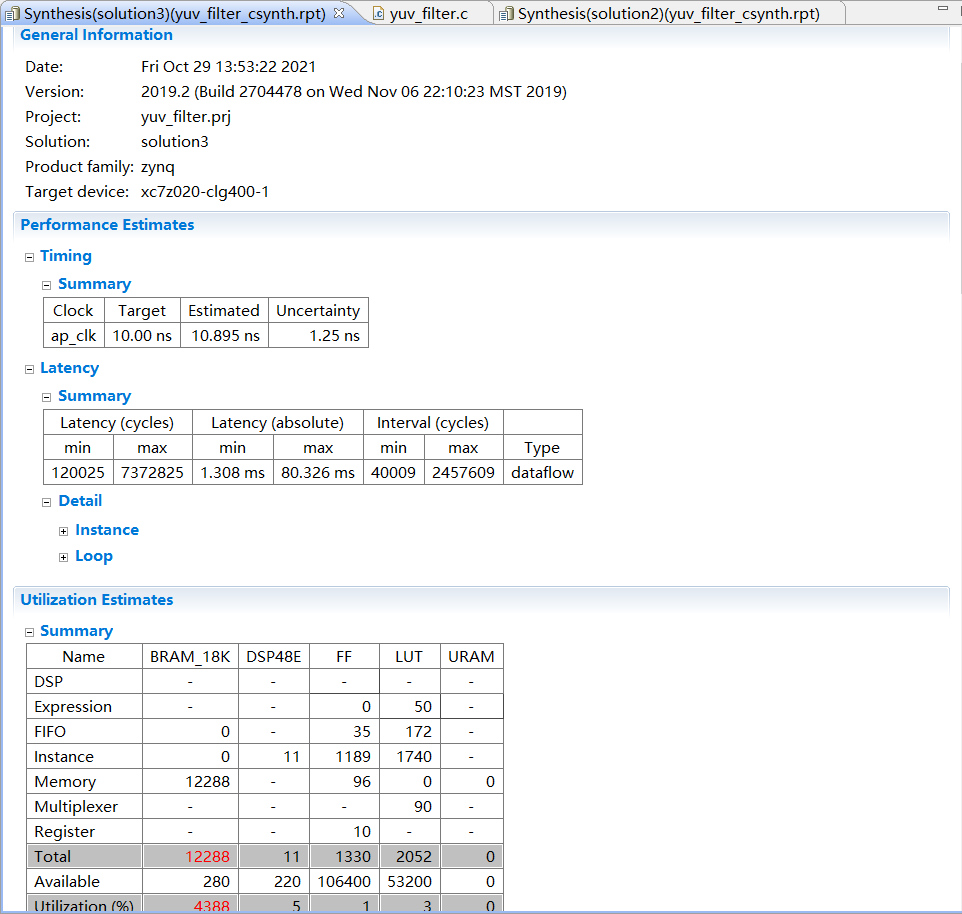
\includegraphics[width=1\textwidth]{5.png}
    \caption{In 2.5, Step 10, a screenshot of the Utilization Estimates.}
\end{figure}
The number of BRAMs required has doubled.

Apply Dataflow configuration command, generate the solution, and observe the improved resources utilization.
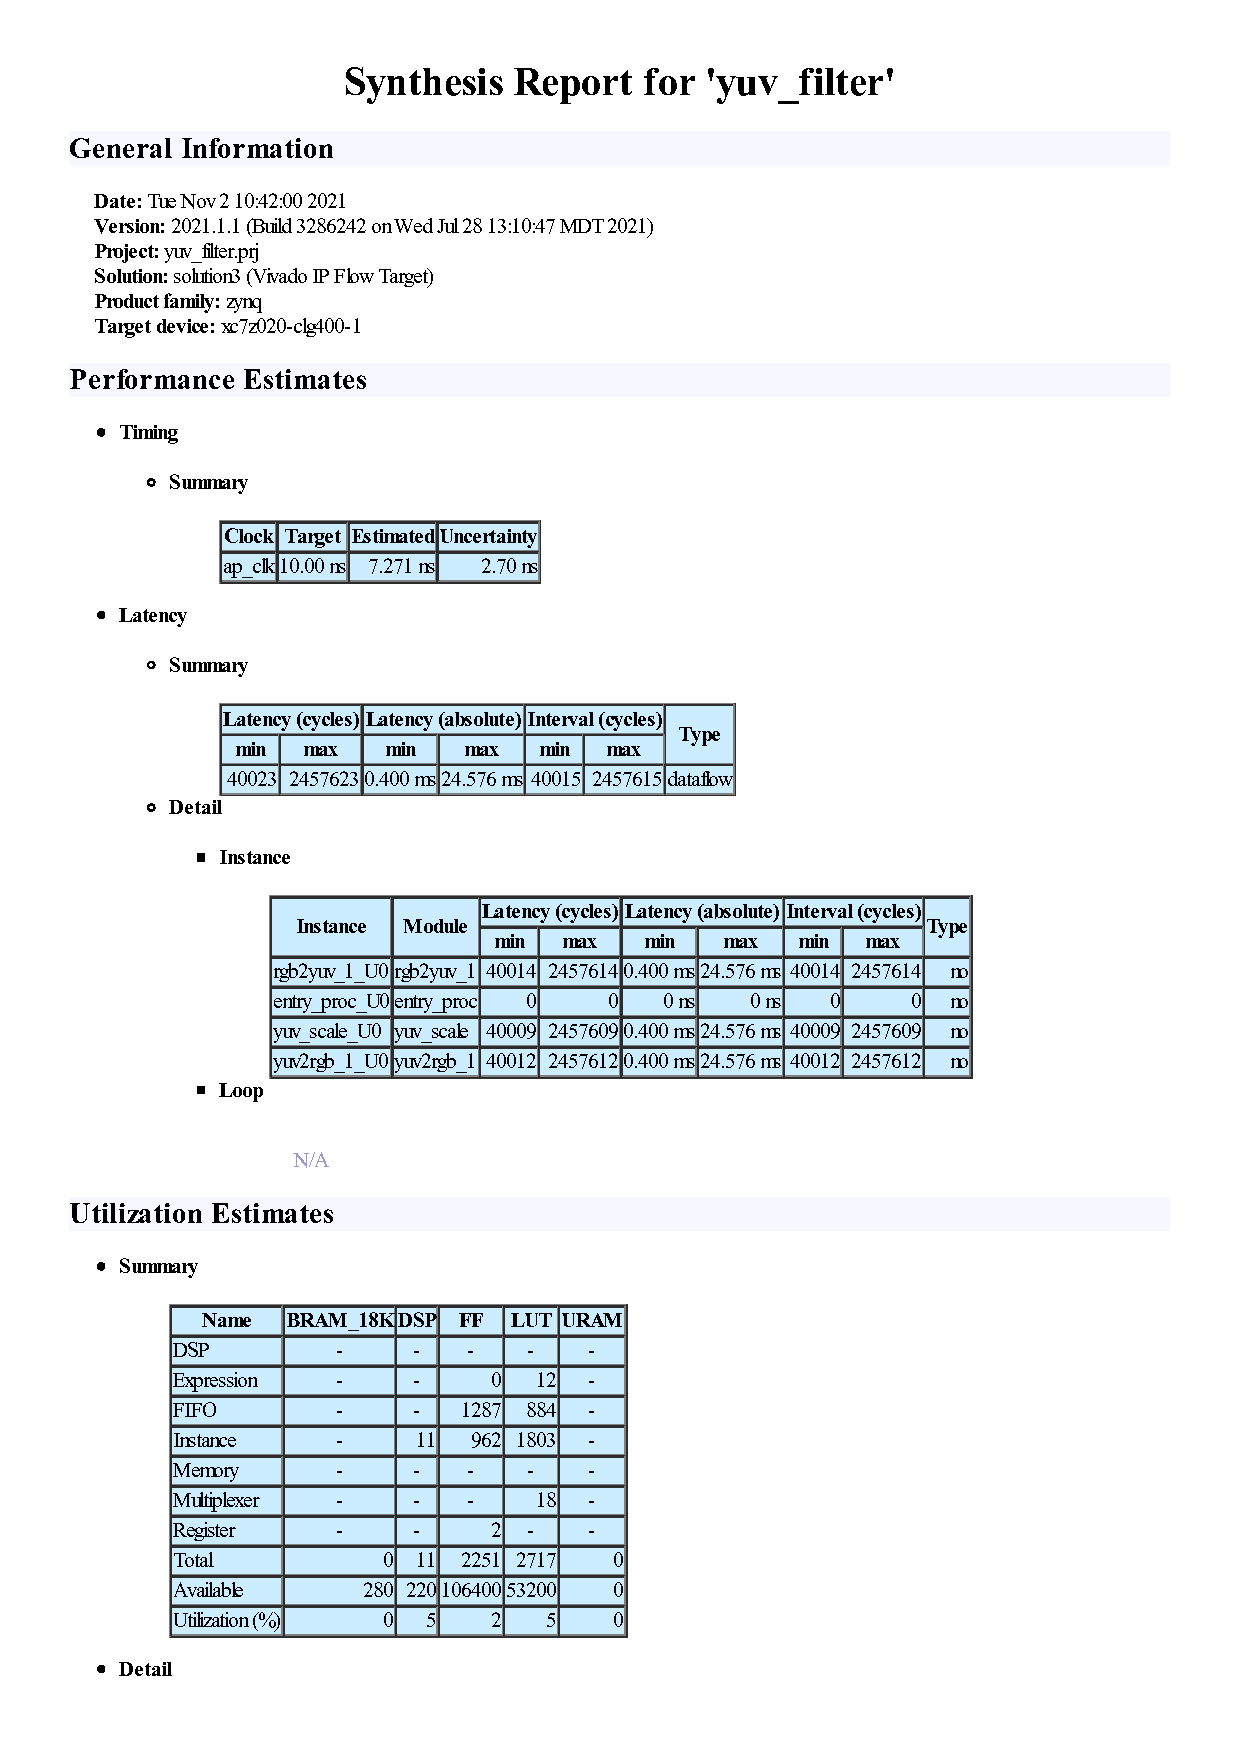
\includepdf[pages=1-4]{solution3_yuv_filter_dataflow_csynth.pdf}
\begin{figure}[H]
    \centering
    
\includegraphics[width=1\textwidth]{6.png}
    \caption{In 2.5, Step 7, a screenshot of synthesis report.}
\end{figure}
The performance parameter has not changed; however, resource estimates show that the design is not using any BRAM. For Vivado HLS 2019.2, other resources (FF, LUT) usage has also reduced.
\subsection{Export and Implement the Design in Vivado HLS}
Vitis HLS 2021.1 Report (RTL Synthesis) and Report (Place \& Route)
\begin{figure}[H]
    \centering
    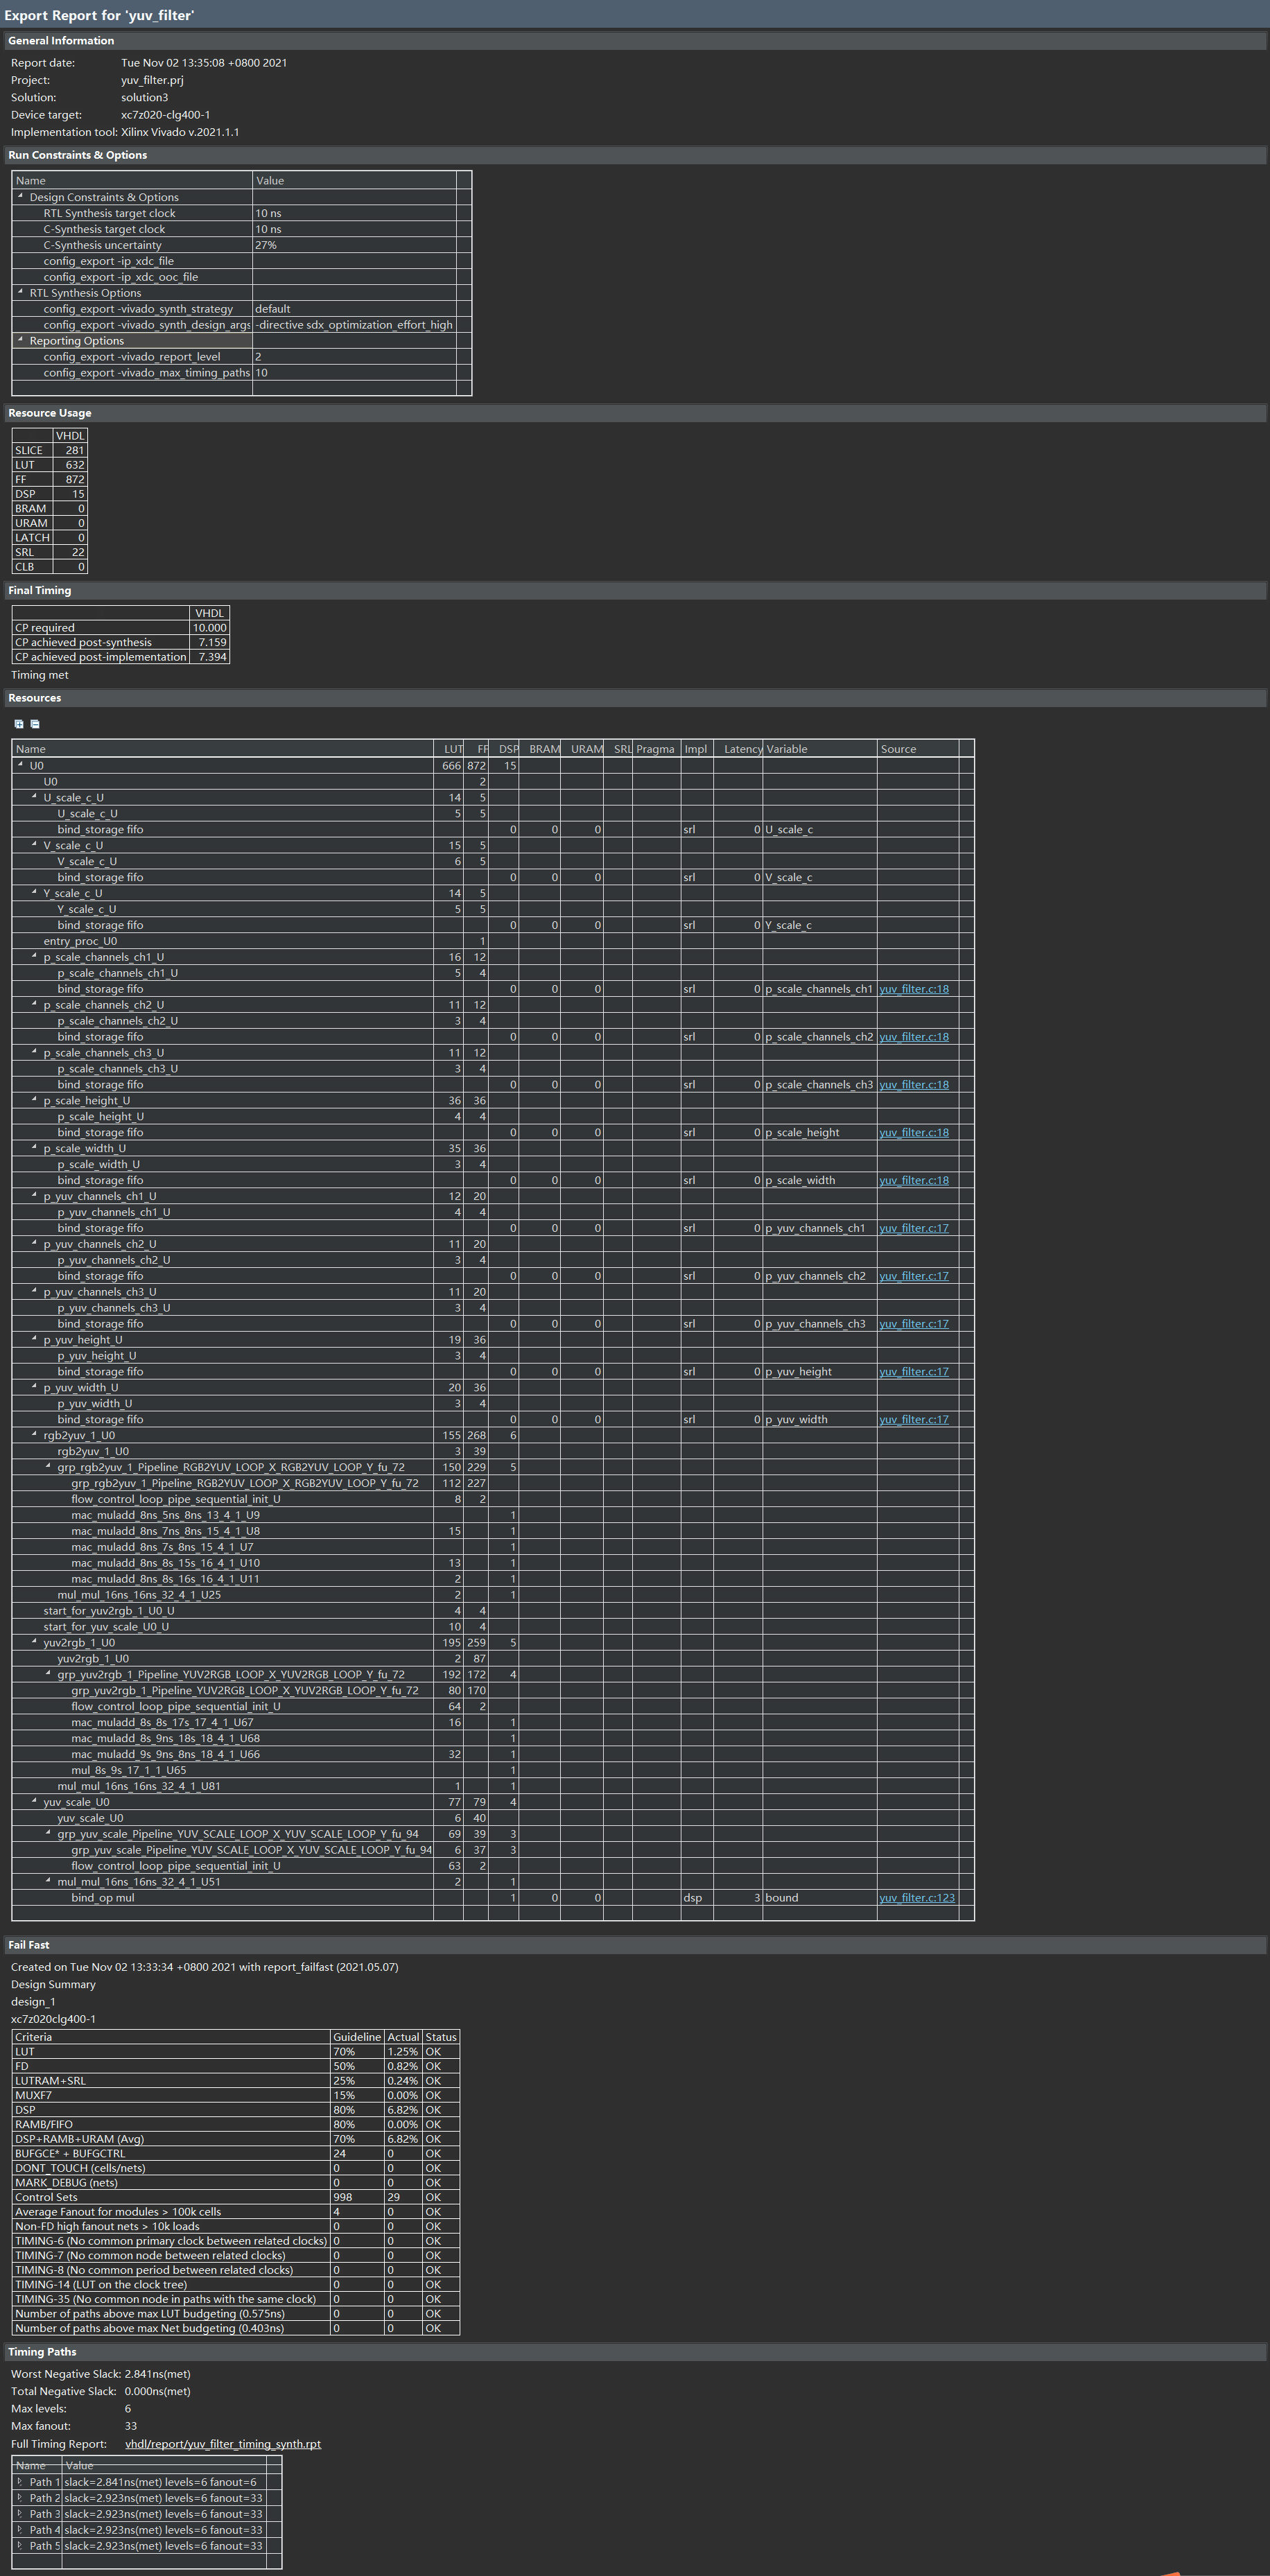
\includegraphics[width=0.9\textwidth]{8.png}
    \caption{Implementation(RTL Synthesis)(solution3)(yuv\_filter\_export.rpt).}
\end{figure}
\begin{figure}[H]
    \centering
    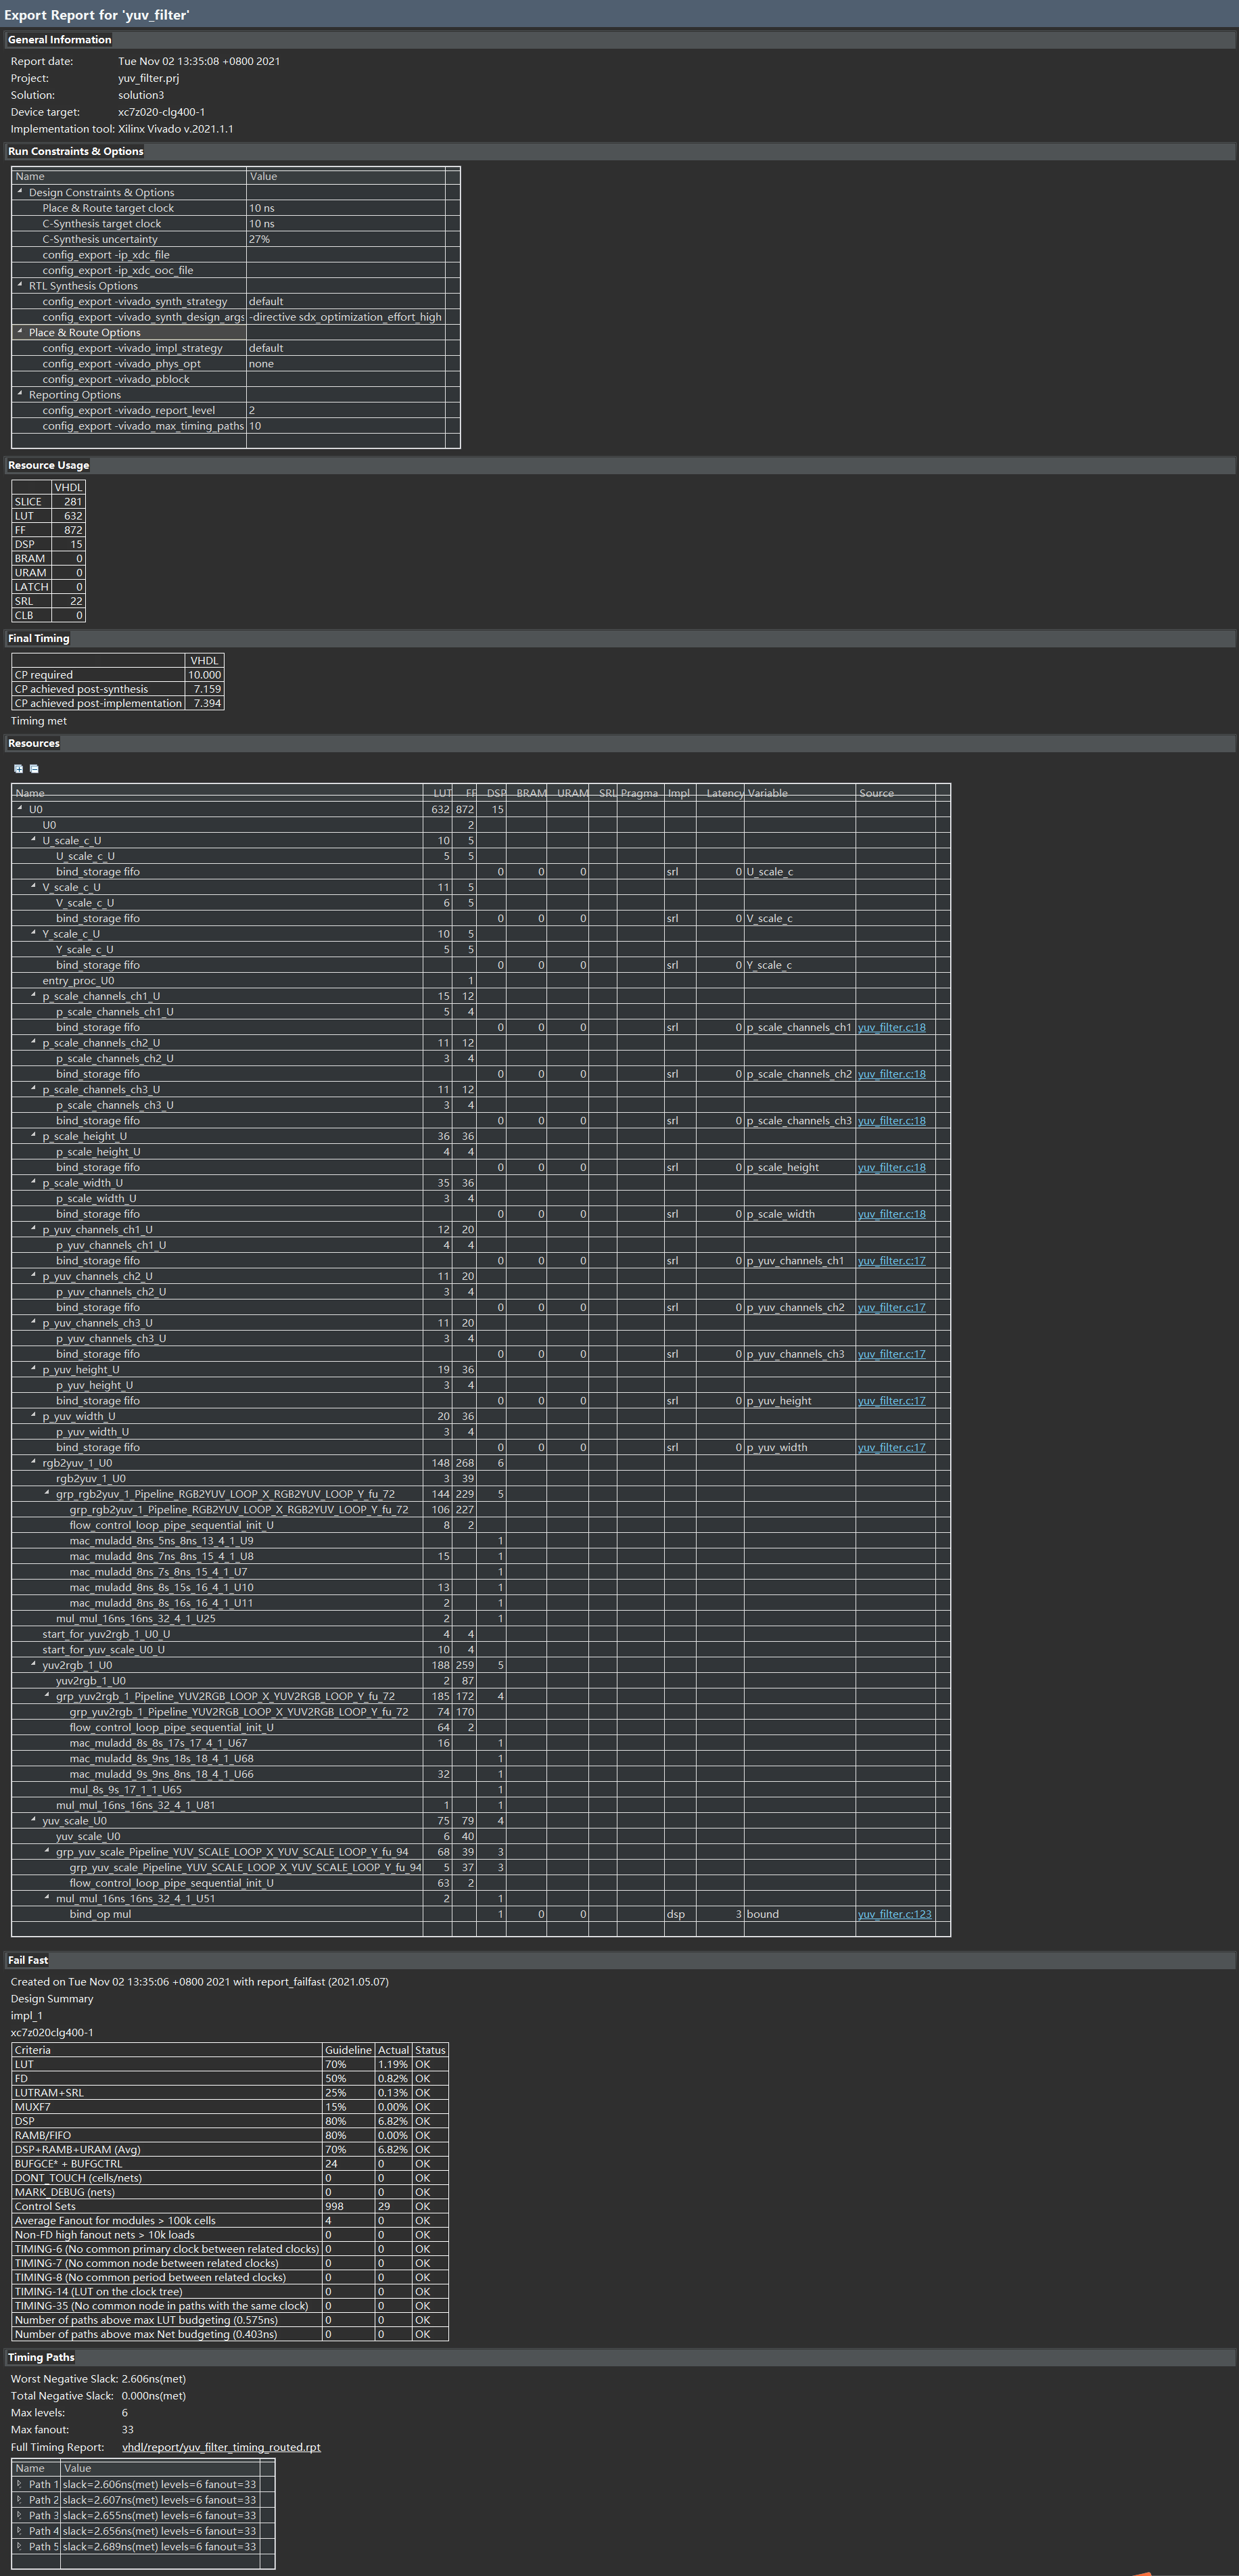
\includegraphics[width=0.9\textwidth]{9.png}
    \caption{Implementation(Place \& Route)(solution3)(yuv\_filter\_export.rpt).}
\end{figure}
Vivado HLS 2019.2:
\begin{figure}[H]
    \centering
    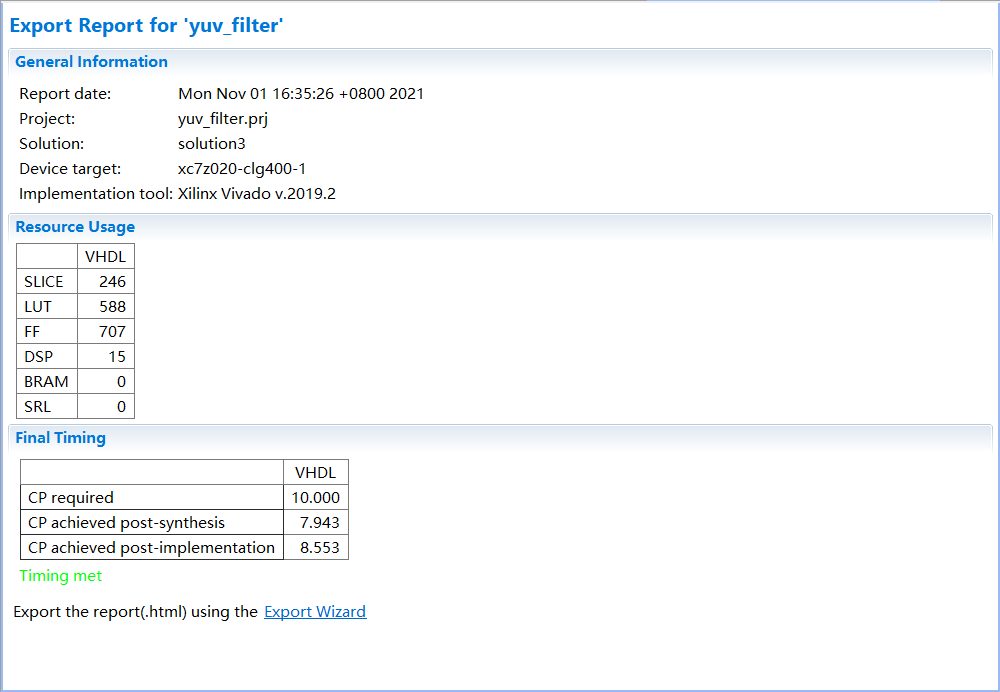
\includegraphics[width=1\textwidth]{7.png}
    \caption{In 2.6, a screenshot of our implementation report.}
\end{figure}
\section{Questions}
\begin{itemize}
    \item Does the pipelining approach employed in this lab apply to all designs? If not, why?
    
    From our perspective, the pipelining approach indeed can be applied into many designs. For instance, for loops without dependencies each other, applying PIPELINE directive can parallel data and decrease the latency and interval. Applying DATAFLOW directive to functions with dependencies can also increase the throughput. However, these methodologies have some limitations. For pipelining and unrolling loops, these loops must have fixed bounds, and PIPELINE directive must be applied into the inner-most loop. For those loops without fixed bounds, this method may not work.
    
    \item In general, how do you identify the performance bottleneck? (You can answer at a high level, based on this lab)
    
    The performance bottleneck should be identified case by case. For instance, a serial execution program may have limited performance. By pipelining method, its performance can be improved. For programs with long loops executed many times, this iteration process may takes a lot of time and become the bottleneck. We can also unroll loops, having several many loops executing concurrently, so that this bottleneck is overcame.
\end{itemize}
\end{document}
